\begin{surferPage}[Singularitat A3+-]{Una singularitat $A_3^{+-}$}
La seva equació, $x^4+y^2-z^2=0$, és similar a la de $A_2^{+-}$,
$x^3+y^2-z^2$,
amb la diferència que és també simètrica respecte del pla $yz$,
ja que
    \[(-x)^4+y^2-z^2=x^4+y^2-z^2.\]
És, doncs, simètrica respecte dels tres plans de coordenades, ja que
$y\mapsto -y$ (respectivament $z\mapsto -z$) no canvia l'equació.

Com per a la tassa de cafè, podem veure una singularitat
$A_3^{+-}$ quan la llum solar travessa un vas de te:
    \vspace*{0.5ex}
    \begin{center}
      \begin{tabular}{c@{\qquad}c}
        \begin{tabular}{@{}c@{}}
          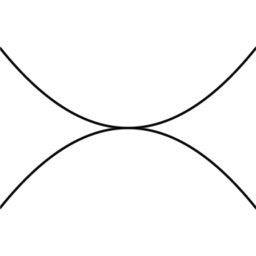
\includegraphics[width=1.4cm]{../../common/images/A3pm_cut_rot}
        \end{tabular}
        &
        \begin{tabular}{@{}c@{}}
          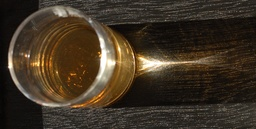
\includegraphics[height=1.4cm]{../../common/images/teeglas_detail}
        \end{tabular}
      \end{tabular}
    \end{center}
    \vspace*{0ex}
La deformació en dues singularitats còniques (que és possible segons
s'ha explicat en el text de la singularitat $A_2^{+-}$),
té l'aspecte següent:
    %
    \begin{center}
      \begin{tabular}{@{}c@{\quad}c@{\quad}c@{}}
        \begin{tabular}{@{}c@{}}
          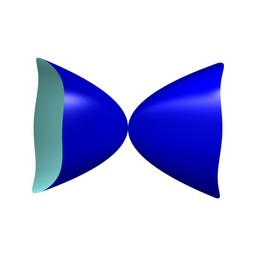
\includegraphics[width=1.2cm]{../../common/images/A3pm_0}
        \end{tabular}
        &
        \begin{tabular}{@{}c@{}}
          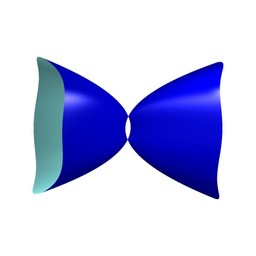
\includegraphics[width=1.2cm]{../../common/images/A3pm_1}
        \end{tabular}
        &
        \begin{tabular}{@{}c@{}}
          
\includegraphics[width=1.2cm]{../../common/images/A3pm_2}
        \end{tabular}
      \end{tabular}
    \end{center}
 
\end{surferPage}
